% 
% 	ondas_planas_raio.tex (LATEX)
% 
% 	Objetivo: Estudo sobre básico da teoria do raio.
%
%	Versão 1.0
% 
% 	Programador: Rodolfo A. C. Neves (Dirack) 23/01/2020
% 
%	Licensa: Software de uso livre e gratuito.

\documentclass[a4paper, 12pt]{article}

% Pacotes fundamentais
  \usepackage{multirow}
  \usepackage[top=2cm, bottom=2cm, left=2.5cm, right=2.5cm]{geometry}
  \usepackage[utf8]{inputenc}
  \usepackage{amsmath, amsfonts, amssymb}
  \usepackage{float}
  \usepackage{graphicx}
  \usepackage[portuguese]{babel}

\begin{document}

\section{A teoria do raio em um modelo de ondas planas}

\begin{figure}[H]
\caption{Exemplo esquemático de uma onda plana atingindo a superfície de aquisição formando um ângulo $\theta$
com a normal à superfície. Apresentamos dois instantâneos da propagação da onda plana, $t$ e $t + \Delta t$.
A velocidade do meio é constante e igual a $v$.}
\begin{center}
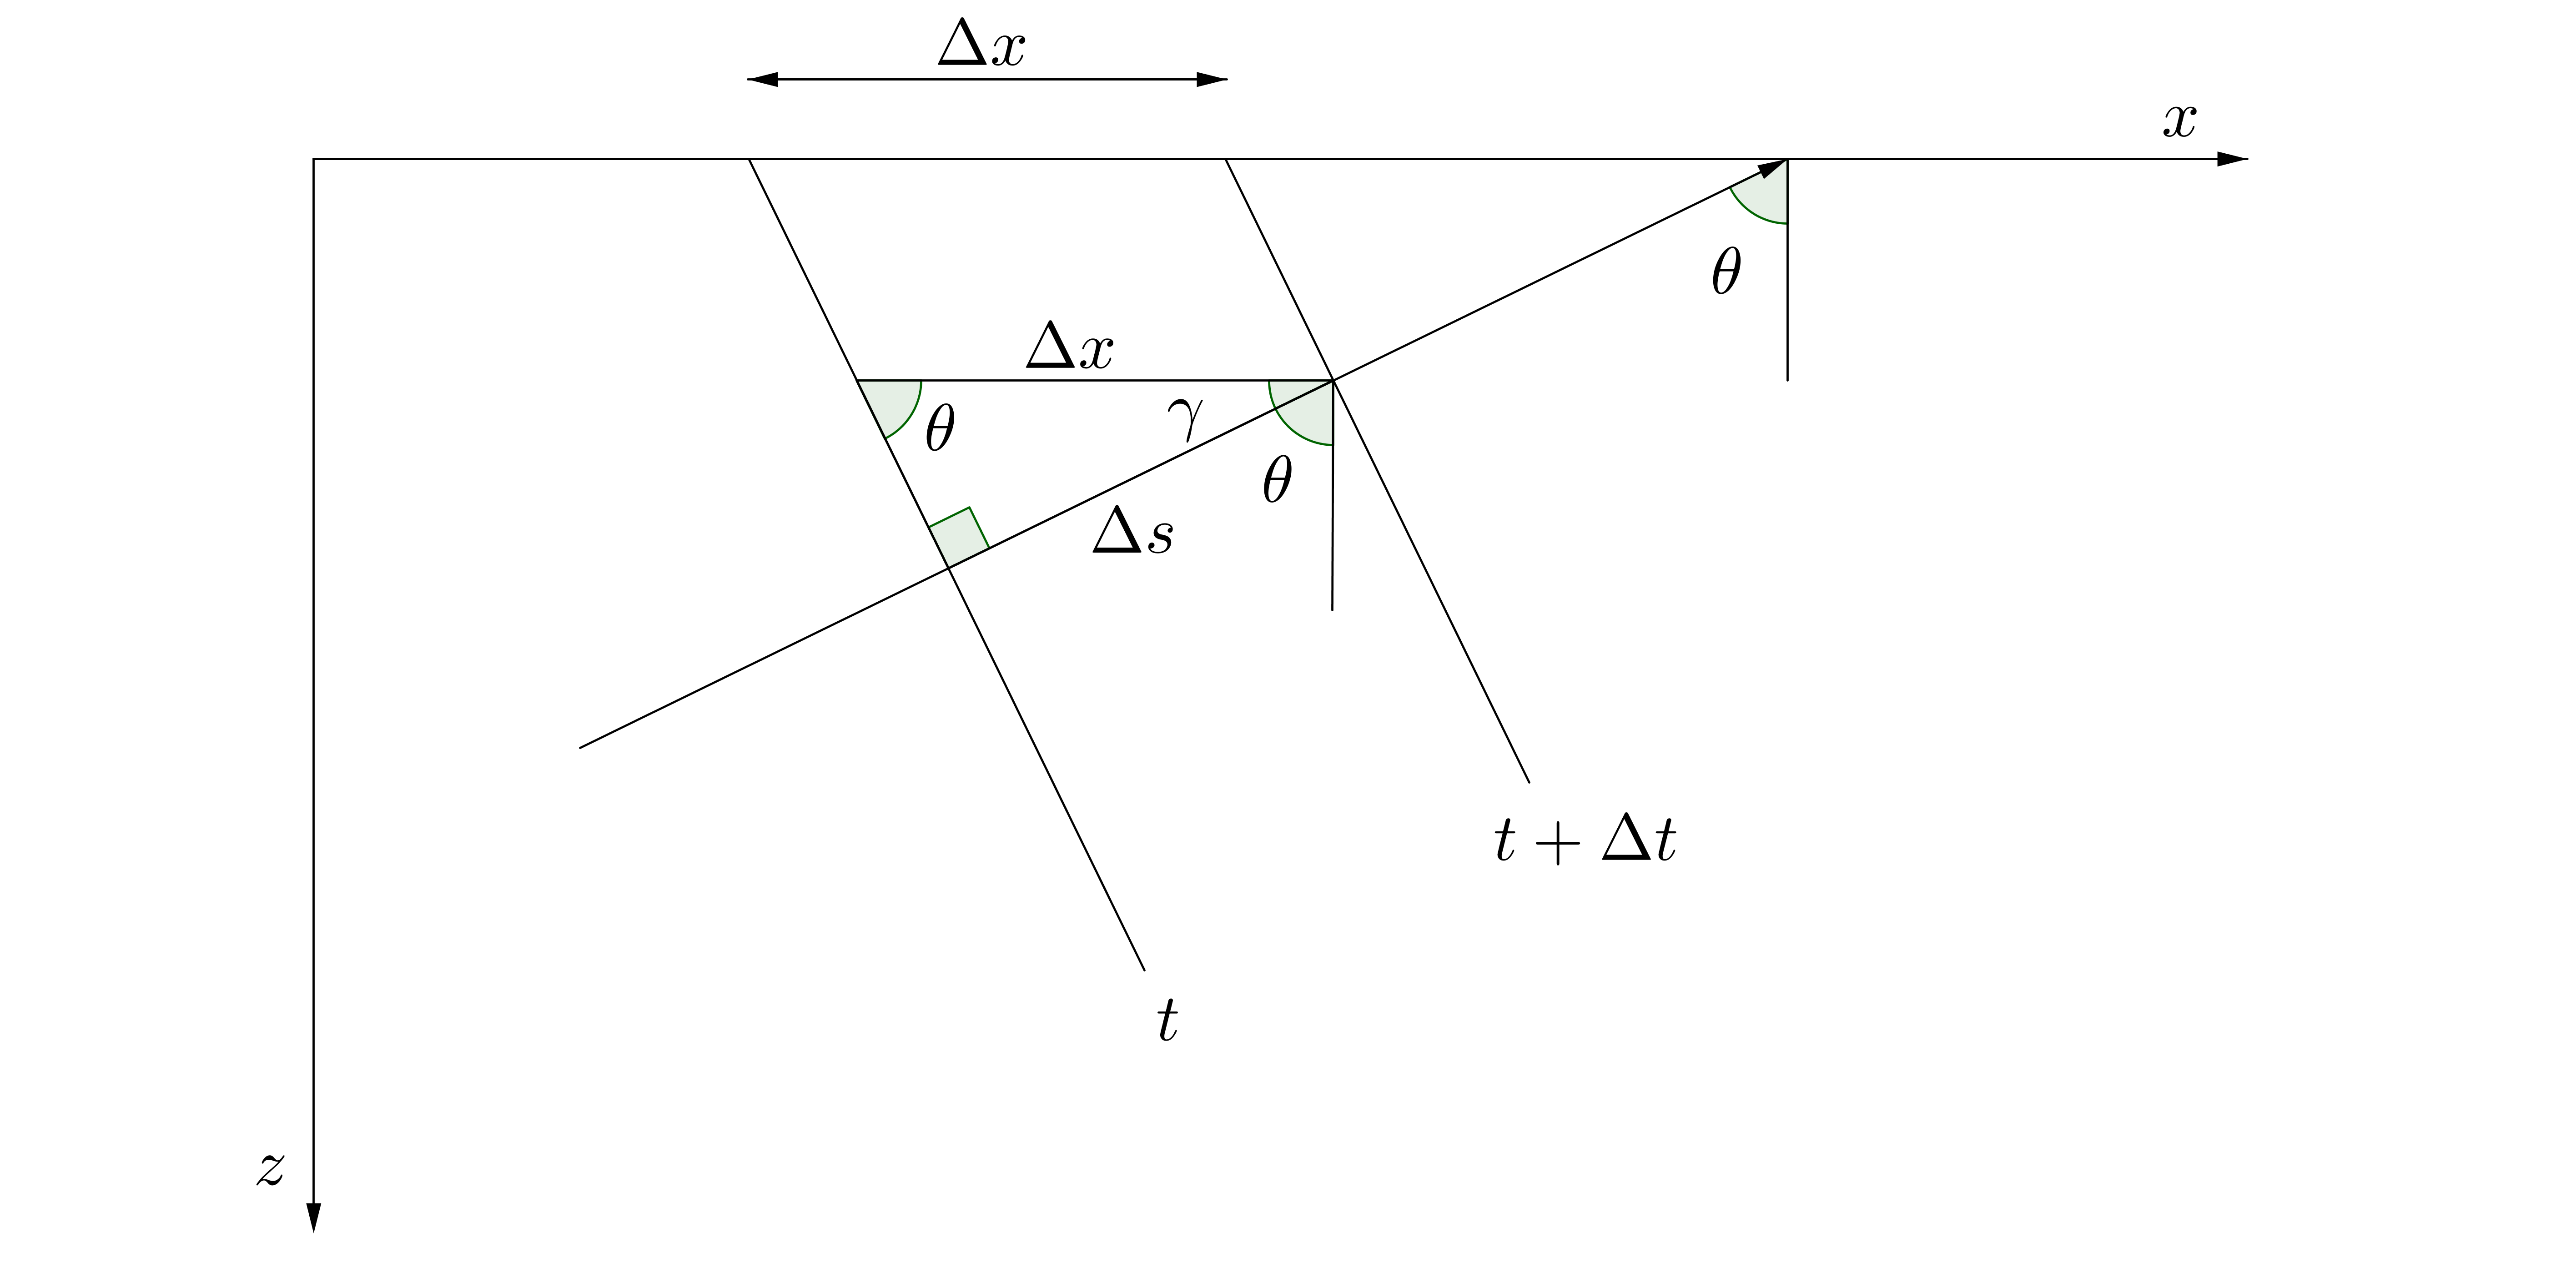
\includegraphics[scale=0.7]{images/raio_ondas_planas.png}
\vspace{-0.3cm}
\end{center}
\begin{center}
 Fonte: Do Autor.
\end{center}
\label{fig:1.1}
\end{figure}

A expressão genérica do sobretempo normal do CRE:

\begin{equation}
\label{eq:1.1}
\tau = \tau_0 + \Delta \tau_{CRE}
\end{equation}

Onde:

\begin{equation}
\label{eq:1.2}
\Delta \tau_{CRE} = \Delta \tau_s + \Delta \tau_g
\end{equation}

Definindo:

\begin{equation}
\label{eq:1.3}
-\Delta x_s = x_s - x_0
\end{equation}

\begin{equation}
\label{eq:1.4}
\Delta x_g = x_g - x_0
\end{equation}

Definindo os tempos $\Delta \tau_s$ e $\Delta \tau_g$ a partir da geometria na Figura \ref{fig:1.1}:

\begin{equation}
\label{eq:1.5}
\Delta \tau_s = \left( \frac{\overline{\hat{C_0}S}}{v_0} - \frac{\overline{\hat{C_0}x_0}}{v_0} \right)
\end{equation}

\begin{equation}
\label{eq:1.6}
\Delta \tau_g = \left( \frac{\overline{\hat{C_0}G}}{v_0} - \frac{\overline{\hat{C_0}x_0}}{v_0} \right)
\end{equation}



\end{document}